\documentclass[journal,12pt,onecolumn]{IEEEtran}
\usepackage{cite}
 \usepackage{caption}
\usepackage{graphicx}
\usepackage{amsmath,amssymb,amsfonts,amsthm}
\usepackage{algorithmic}
\usepackage{graphicx}
\usepackage{textcomp}
\usepackage{xcolor}
\usepackage{txfonts}
\usepackage{listings}
\usepackage{enumitem}
\usepackage{mathtools}
\usepackage{gensymb}
\usepackage{comment}
\usepackage[breaklinks=true]{hyperref}
\usepackage{tkz-euclide} 
\usepackage{listings}
\usepackage{gvv}
%\def\inputGnumericTable{}                                 
\usepackage[latin1]{inputenc} 
\usetikzlibrary{arrows.meta, positioning}
\usepackage{xparse}
\usepackage{color}                                            
\usepackage{array}                                            
\usepackage{longtable}                                       
\usepackage{calc}                                             
\usepackage{multirow}
\usepackage{multicol}
\usepackage{hhline}                                           
\usepackage{ifthen}                                           
\usepackage{lscape}
\usepackage{tabularx}
\usepackage{array}
\usepackage{float}

\usepackage{float}
%\newcommand{\define}{\stackrel{\triangle}{=}}
\theoremstyle{remark}
\usepackage{circuitikz}
\captionsetup{justification=centering}
\usepackage{tikz}

\title{Matrices in Geometry 1.5.25}
\author{EE25BTECH11037 - Divyansh}
\begin{document}
\vspace{3cm}
\maketitle
{\let\newpage\relax\maketitle}
\textbf{Question: }
In what ratio does the point \myvec{\frac{24}{11} \\ y} divide the line segment joining the points \textbf{P}=\myvec{2 \\ -2} and \textbf{Q}=\myvec{3 \\ 7}? Also find the value of y.\\

\textbf{Given: } 
$\vec{P}=\myvec{2\\-2}$, $\vec{Q}\myvec{3\\7}$ and a point $\vec{R} \myvec{\frac{24}{11} \\ y}$ on $PQ$.

Let $R$ divide $PQ$ internally in the ratio $k:1$.\\
Therefore, they are defined to be collinear if rank of the collinearity matrix is 1
\begin{align*}
    \text{Collinearity matrix is }\myvec{\vec{P}- \vec{R} & \vec{Q}-\vec{R}}^{\top}=1\\
    \vec{P}-\vec{R}=\myvec{\dfrac{-2}{11} \\ -y-2}\\
    \vec{Q}-\vec{R}=\myvec{\dfrac{9}{11} \\ 7-y}\\
    \implies \text{rank}\myvec{\frac{-2}{11} & -y-2 \\ \frac{9}{11} & 7-y} = 1\\
    \myvec{\frac{-2}{11} & -2-y \\ \frac{9}{11} & 7-y}\overset{R_2 \rightarrow R_2 + \frac{9}{2}R_1}{\longrightarrow} \myvec{\frac{-2}{11} & -2-y \\ 0 & \dfrac{-11-4y}{2}}\\
    \text{for rank of this matrix to be 1, all the elements in the lower row have to be zero}\\
    \therefore -11-4y=0 \implies
    y=\dfrac{-4}{11}
\end{align*}
We know that $k$ is the ratio in which $\vec{R}$ divides $\vec{P}$ and $\vec{Q}$,
\begin{align*}
   \vec{R}=\dfrac{k\vec{Q}+\vec{P}}{1+k}\\
   k\brak{\vec{R}-\vec{Q}}&= \vec{P}-\vec{R}\\
   \implies k =\dfrac{\brak{\vec{P}-\vec{R}}^{\top}\brak{\vec{R}-\vec{Q}}}{\norm{\vec{R}-\vec{Q}}^2}\\
   \brak{\vec{P}-\vec{R}}^{\top}=\myvec{\frac{-2}{11} & \frac{-18}{11}}\\
   \brak{\vec{R}-\vec{Q}}=\myvec{\frac{-9}{11} \\ \frac{-81}{11}}\\
   \norm{\vec{R}-\vec{Q}}^2=\myvec{\vec{R}-\vec{Q}}^{\top} \myvec{\vec{R}-\vec{Q}}\\=\myvec{\frac{-9}{11} & \frac{-81}{11}}\myvec{\frac{-9}{11} \\ \frac{-81}{11}}=\frac{81}{121} + \frac{6561}{121}=\frac{6642}{121}\\
   \therefore k=\dfrac{\myvec{\frac{-2}{11} & \frac{-18}{11}}\myvec{\frac{-9}{11} \\ \frac{-81}{11}}}{\frac{6642}{121}}\\
   \end{align*}
\begin{align*}
   \implies k=\dfrac{\frac{18}{121} + \frac{1458}{121}}{\frac{6642}{121}}
   \implies k=\dfrac{1476}{6624}=\dfrac{2}{9}
\end{align*}

\begin{align*}
 \text{Hence, the final answer is }\fbox{k = \dfrac{2}{9}} \; \text{and} \; \fbox{y = \dfrac{-4}{11}}  
\end{align*}
\begin{figure}[H]
    \centering
    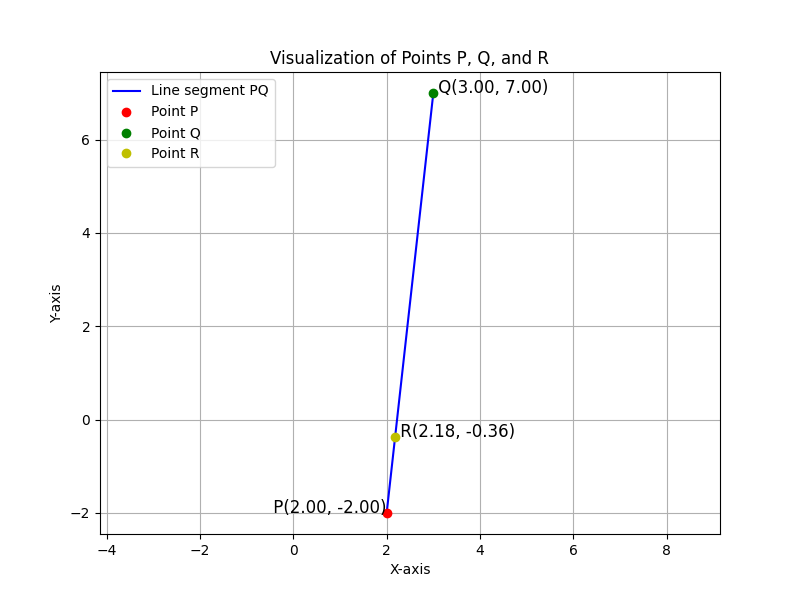
\includegraphics[width=1\columnwidth]{figs/1.png}
    \caption{Plot for 1.5.25}
    \label{fig:placeholder}
\end{figure}
\end{document}